\documentclass{beamer}
\usepackage[latin1]{inputenc}
\usefonttheme[onlylarge]{structurebold}
\setbeamerfont*{frametitle}{size=\normalsize,series=\bfseries}
\setbeamertemplate{navigation symbols}{}
\usetheme{Goettingen}

\title[Journal Club 1]{Synthetic gene expression perturbation systems with rapid, tunable, single-gene specificity in yeast}
\author{R. Scott McIsaac\inst{1}\inst{2}, Benjamin L. Oakes\inst{1}, Xin Wang\inst{1}\inst{3}, Krysta A. Dummit\inst{1}, David Botstein\inst{1}\inst{3} and Marcus B. Noyes\inst{1}}
\institute{
\inst{1}%
The Lewis-Sigler Institute for Integrative Genomics, Princeton University
\and \vskip-2mm \inst{2}%
Graduate Program in Quantitative and Computational Biology, Princeton University
\and \vskip-2mm \inst{3}%
Department of Molecular Biology, Princeton University
}
\date[]{Carles Boix}
\begin{document}

\begin{frame}
\titlepage
\end{frame}
%------------------ %------------------ %------------------ %------------------ %------------------ %------------------ 
\section{Background}
\begin{frame}{Background}
    \begin{itemize}
        \item<1-> System to perturb the expression of a single gene only.
            \bigskip
        \item<2-> Tool to understand complex regulatory networks.
            \bigskip
        \item<3-> Nutritional perturbation, such as GAL or MET promoters.
            \bigskip
        \item<4-> Use inducers that don't have any other influence on the system.
            \bigskip
        \item<5-> Use DBDs that do not have multiple locations in the genome ($\sim 9$ bp)
    \end{itemize}
\end{frame}

\begin{frame}
    Create a system which is:
    \begin{itemize}
        \item[] Fast
        \item[] Tightly regulated
        \item[] Gratuitous (no effect on other genes)
        \item[] Gradable
    \end{itemize}
    \pause
    \bigskip
    \bigskip
    This is the $\beta$-estradiol system which we are using.
    \begin{itemize}
        \item[] DNA-binding domain (DBD)
        \item[] Human estrogen receptor (ER) 
        \item[] VP16 activation domain
        \item[] Use specific zinc fingers (Z$_3$ and Z$_4$)
    \end{itemize}
\end{frame}

\begin{frame}
    \begin{figure}[!ht]
        \begin{center}
        {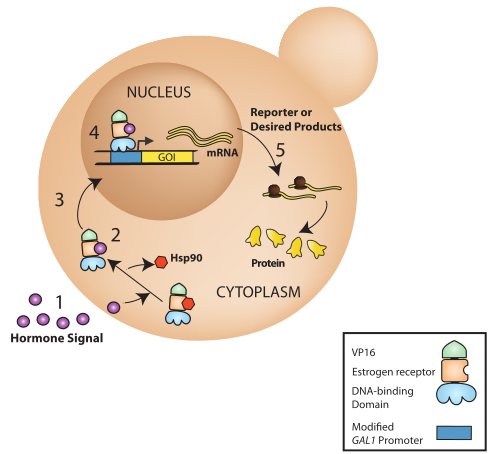
\includegraphics[width=0.7\textwidth]{McIsaacfig1.png}}
        \caption{Synthesized ATF system}
        \label{fig:Curve1}
    \end{center}
\end{figure}
\end{frame}

%------------------ %------------------ %------------------ %------------------ %------------------ %------------------ %------------------ 
% HERE WE RUN THROUGH A COUPLE OF FIGURES THAT DEMONSTRATE THE SYSTEM.
\section{Results}
\begin{frame}
    \begin{figure}[!ht]
        \centering
        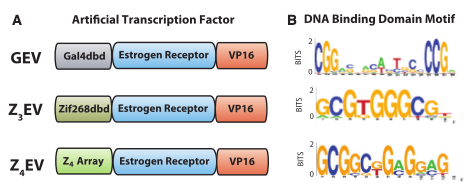
\includegraphics[width=0.7\textwidth]{McIsaacfig2.png}
        \caption{Constructed ATFs and Binding Motifs}
        \label{fig:atfs}
    \end{figure}
    \pause
    \begin{figure}[ht!]
        \centering
        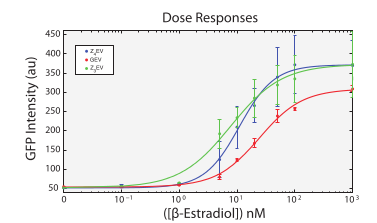
\includegraphics[width=0.6\textwidth]{McIsaacfig3.png}
        \caption{GFP level with reporter plasmid.}
        \label{fig:grade}
    \end{figure}
\end{frame}

\begin{frame}
    \begin{figure}[ht!]
        \centering
        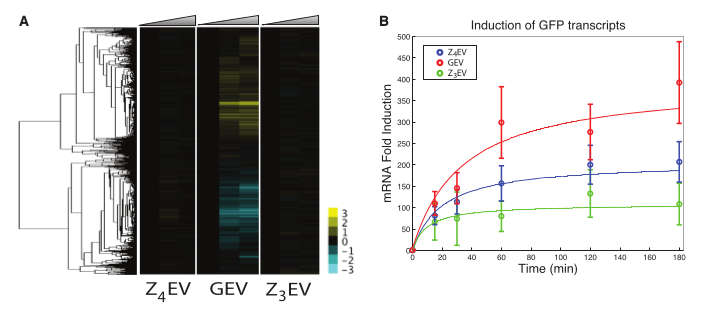
\includegraphics[width=0.8\textwidth]{McIsaacfig4.png}
        \caption{Gene expression levels and GFP mRNA levels.}
        \label{fig:mRNA}
    \end{figure}
    More than 50-fold induction in 15 minutes.
\end{frame}

\begin{frame}
    \begin{figure}[ht!]
        \centering
        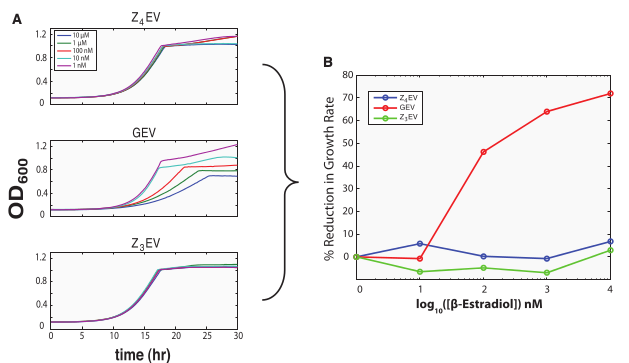
\includegraphics[width=0.8\textwidth]{McIsaacfig5.png}
        \caption{Growth defect present in GEV strains.}
        \label{fig:growthGEV}
    \end{figure}
    Increasing $\beta$-estradiol decreases GEV growth rate.\\
    \textbf{70\%} Growth rate decrease from $10$nM to $10\mu$M.
\end{frame}

\begin{frame}
    \begin{figure}[ht!]
        \centering
        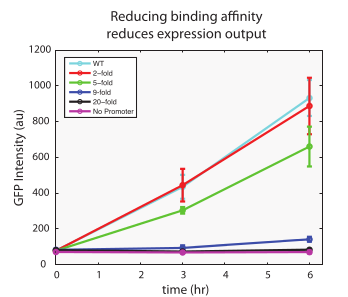
\includegraphics[width=0.6\textwidth]{McIsaacfig6.png}
        \caption{Grading output by binding affinity}
        \label{fig:growthGEV}
    \end{figure}
\end{frame}

\begin{frame}
    \begin{figure}[ht!]
        \centering
        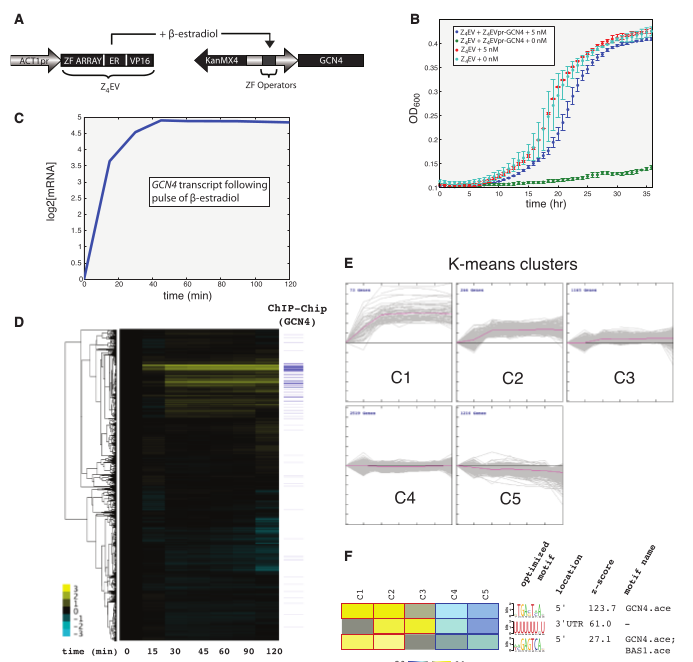
\includegraphics[width=0.7\textwidth]{McIsaacfig7.png}
        \caption{\emph{GCN4} (GOI) is a transcriptional activator of enzymes required for production of \emph{aa}.}
        \label{fig:growthGEV}
    \end{figure}
\end{frame}

%------------------ %------------------ %------------------ %------------------ %------------------ %------------------ %------------------ 
\section{Conclusions}
\begin{frame}
    The $\beta$-estradiol system:
    \begin{itemize}
        \item Is gradable
        \item Gratuitous
        \item Fast (50 fold in 15 min)
        \item Does not have a growth defect
        \item Can be moderated by binding affinity % Note I would like to see binding SPECIFICITY of the 20 fold etc.
    \end{itemize}
    \pause
    Have shown utility with a case study: \emph{GCN4}. Authors find $\sim 200-300$ genes repressed and enriched (116 genes known before from ChIP data).
\end{frame}
% TODO future directions??

\end{document}
